\documentclass[a4]{beamer}
%\usepackage[pdftex]{graphicx}
\usepackage[utf8]{inputenc}
\usepackage[english]{babel}
\usepackage[T1]{fontenc}
%\usepackage{mathtools}
%\usepackage{amssymb}
\usepackage{underscore}
\usepackage{wrapfig}
\usepackage{rotating}
\usepackage{multirow}
%\usepackage{wrapfig}
%\usepackage[skip=1.5pt,font=scriptsize]{caption}
%\usepackage{enumitem}
\usetheme{Frankfurt}
\usecolortheme{seahorse}
\setbeamertemplate{frametitle}[default][colsep=-4bp,rounded=false,shadow=false]
\setbeamertemplate{title page}[default][colsep=-4bp,rounded=false,shadow=false]
\addtobeamertemplate{navigation symbols}{}{ \hspace{1em}    \usebeamerfont{footline}%
    \insertframenumber / \inserttotalframenumber }
\setbeamertemplate{itemize items}[circle]

\newcommand{\bofr}{\mathcal{B}(\mathbb{R})}
\newcommand{\RR}{\mathbb{R}}
\newcommand{\bs}{\backslash}
\newcommand{\NN}{\mathbb{N}}
\newcommand{\ZZ}{\mathbb{Z}}
\newcommand{\QQ}{\mathbb{Q}}
\newcommand{\BB}{\mathbb{B}}
\newcommand{\CC}{\mathbb{C}}
\newcommand{\FF}{\mathbb{F}}
\newcommand{\la}{\lambda}
\newcommand{\coola}{\mathcal{A}}
\newcommand{\coolm}{\mathcal{M}}
\newcommand{\cooll}{\mathcal{L}}
\newcommand{\ipl}{\langle}
\newcommand{\ipr}{\rangle}
\newcommand{\limn}{\lim_{n \to \infty}}
\newcommand{\eq}[1]{\begin{align*} #1 \end{align*}}
\newcommand{\lr}{\Leftrightarrow}
\newcommand{\set}[1]{\left\lbrace #1 \right\rbrace}
\renewcommand{\d}{\,\text{d}}
\newcommand{\pt}[1]{\left(#1\right)}
\newcommand{\fork}[1]{\left\{\begin{array}{lr}#1\end{array}\right.} % gaffel-funktion
\newcommand{\tuad}[1]{\qquad\ \text{#1}\ }
\newcommand{\ND}{\mathcal{N}}
\newcommand{\Perp}{\perp \! \! \! \perp}
\newcommand{\ddu}{\frac{\partial}{\partial u}}
\newcommand{\ddv}{\frac{\partial}{\partial v}}
\newcommand{\ddx}{\frac{\partial}{\partial x}}
\newcommand{\dds}{\frac{\partial}{\partial s}}
\newcommand{\ddt}{\frac{\partial}{\partial t}}
\newcommand{\dd}{\partial}
\newcommand{\red}[1]{\textcolor{red}{#1}}
\newcommand{\blue}[1]{\textcolor{blue}{#1}}
\newcommand{\var}[1]{\textsc{\lowercase{#1}}}


%\newenvironment{myindentpar}[1]%
%	{\begin{list}{}%
%             {\setlength{\leftmargin}{#1}}%
%             \item[]%
%     }
%    {\end{list}}

\DeclareMathOperator*{\plimo}{plim}
\DeclareMathOperator*{\cov}{cov}
\DeclareMathOperator*{\E}{E}
\DeclareMathOperator*{\V}{V}
\DeclareMathOperator*{\T}{T}
\newcommand{\plim}{\plimo_{n \to \infty}}
\usepackage{wallpaper}
%\definecolor{blue(pigment)}{rgb}{0.2, 0.2, 0.6}
%\definecolor{darkcerulean}{rgb}{0.03, 0.27, 0.49}
%\setbeamercolor{frametitle}{bg=blue(pigment)}

%\begin{center}
%\includegraphics[scale=0.3]{residualplot_logengel.jpeg} 
%\end{center} 
 
\title{Exploratory data structure comparisons}
\subtitle{A few tools based on PCA}
\author{Anne H. Petersen, Bo Markussen \& Karl Bang Christensen}
\date{March 15, 2017}
 
\begin{document}
\maketitle

\section{Set-up}

\subsection{Problem}
\begin{frame}
\frametitle{Problem}
\begin{itemize}
\item Let $X_k$ be a $n_k \times d$ matrix of data for $k \in \{1, 2\}$ with (the same) ordinal or numeric variables for both $k$. 
\item We ask: Are the structures of $X_1$ and $X_2$ similar? Can we e.g. combine the two into one dataset $X = \begin{pmatrix} X_1 \\ X_2 \end{pmatrix}$ with $n = n_1 + n_2$ observations of the $d$ variables without problems?
\item Example: $X_1$ stems from a survey administered by telephone, $X_2$ stems from the same survey administered as a web questionnaire. Can we analyze the "full" dataset jointly?
\item Example: $X_1$ represents data from a study conducted in Denmark, $X_2$ represents the same measurements from a study in Bulgaria. Can we combine the two?
\end{itemize}
\end{frame}

\subsection{Requirements}
\begin{frame}
\frametitle{Requirements for a candidate method}
\begin{itemize}
\item New origin stories of datasets add a new challenge to this question: Increasingly often, data is \textit{not} collected with a specific endpoint in mind (e.g. PISA, the European Social Survey (ESS), traffic data from websites, ...)
	\begin{itemize}
		\item[$\Rightarrow$] We wish to answer the question \textit{before} specifying what we are going to use the data for
	\end{itemize}
\item In particular, we do not want to specify a model (yet) 
	\begin{itemize}
		\item[$\Rightarrow$] Cannot use e.g. IRT methods, regression methods  
	\end{itemize}
\item We do not want just a test, but instead tools for intuitive, exploratory investigations that might lead to insights as to \textit{why} the differences occur 
\end{itemize}
\end{frame}

\subsection{Strategy}
\begin{frame}
\frametitle{Solution strategy}
\begin{itemize}
\item Focus on the covariance structures:
\begin{itemize}
\item Let $S_1 = \tilde{\V}(X_1)$ and $S_2 = \tilde{\V}(X_2)$ denote the empirical covariance matrices of the two datasets
\item $S_k$ describes the interplay between variables. And for Gaussian (zero-mean) variables: A sufficient statistic for the joint distribution.
\item In principle, we could compare $S_1$ and $S_2$ entry by entry, but this strategy does not scale well
\end{itemize}
\item Deconstruct each covariance matrix such that we can deal with the most informative components first and ignore noise
\begin{itemize}
\item[$\rightarrow$] Use Principal Component Analysis (PCA)
\end{itemize}
\end{itemize}
\end{frame}

\section{PCA}

\begin{frame}
\frametitle{Principal component analysis: A greedy interpretation}
\begin{itemize}
\item Let $U \subset \RR^d$ be the set of unit vectors of dimension $d$. For $j \in 1, ..., d$, define: 
\begin{itemize}
\item[] The $j$th \textit{loading vector}: \onslide<2->{\blue{(eigenvectors)}}
$$\eta_j := \text{argmax}_{u \in U: u \perp \hat{K}_{j-1}} \tilde{\V}(u^\top X^\top)$$
\item[] The $j$th \textit{variance component}: \onslide<2->{\blue{(eigenvalues)}}
$$\lambda_j := \tilde{\V}(\eta_j^\top X^\top)$$
\end{itemize}
where $K_0 = \emptyset$ and $K_j = \text{span}\{\eta_1, ..., \eta_j\}$. 
\item Now, $\eta_1$ is the linear transformation of dimension $d \times 1$ of the data that explains the largest possible amount of the variance, and this amount is $\frac{\lambda_1}{tr{S}}$.
\item It holds that $S = \sum_{j=1}^d \lambda_j \eta_j \eta_j^\top$
\end{itemize}
\end{frame}


\section{PCADSC tools}

\subsection{PCADSC}
\begin{frame}
\frametitle{Principle Component Analysis-based Data Structure Comparisons (PCADSC)}
\begin{itemize}
\item PCADSC: Conduct PCA decomposition on each of the (standardized) datasets $X_1$ and $X_2$ and compare the results
\item We provide three tools for visualizing the results of PCA in order to compare data structures:
	\begin{itemize}
		\item The cumulated eigenvalue (CE) plot \onslide<2->{\blue{- compare eigenvalues}}
		\item The hair plot \onslide<3->{\blue{- explain $S_1$ from $S_2$ (and $S_2$ from $S_1$)}}
		\item The pancake plot \onslide<4->{\blue{- compare loadings}}
	\end{itemize}
\item Available in \texttt{R}-package at \url{www.github.com/AnnePetersen1/PCADSC}
\onslide<5->{\item First step of all procedures:
	\begin{itemize}
		\item[1.]  For $k \in \{1, 2\}$, standardize $X_k$ and perform PCA, thereby obtaining $\eta^k_1, ..., \eta^k_d$ and $\lambda^k_1, ..., \lambda^k_d$
	\end{itemize}}  
\end{itemize}
\end{frame}

\subsection{The CE plot}
\begin{frame}
\frametitle{The CE plot}
\begin{itemize}
\item Let $\lambda_1, ..., \lambda_d$ be the eigenvalues of the covariance matrix of the combined dataset, $X$. 
\item Draw a piecewise linear curve through the points
\begin{align*}
&(0,0), 
(\lambda_1,\lambda^1_1-\lambda^2_1), 
(\lambda_1 + \lambda_2,\lambda^1_1+\lambda^1_2-\lambda^2_1-\lambda^2_2), \\ 
&\ldots, \bigg( \sum_{j=1}^d \lambda_j, \sum_{j=1}^d \lambda^1_j - \lambda^2_j \bigg).
\end{align*}
\item Get an idea of the variability of the results using repeated random splits:
\begin{itemize}
\item E.g. 10000 times, divide $X$ randomly into two subsets of size $n_1$ and $n_2$, respectively and perform the steps from above
\item Draw a shaded region representing a "bootstrapped" pointwise confidence interval obtained in this way
\item Draw a subset of the random curves (e.g. 20) to illustrate how they vary
\end{itemize}
\end{itemize}
\end{frame}

\begin{frame}
\frametitle{The CE plot}
\begin{figure}
\centering
    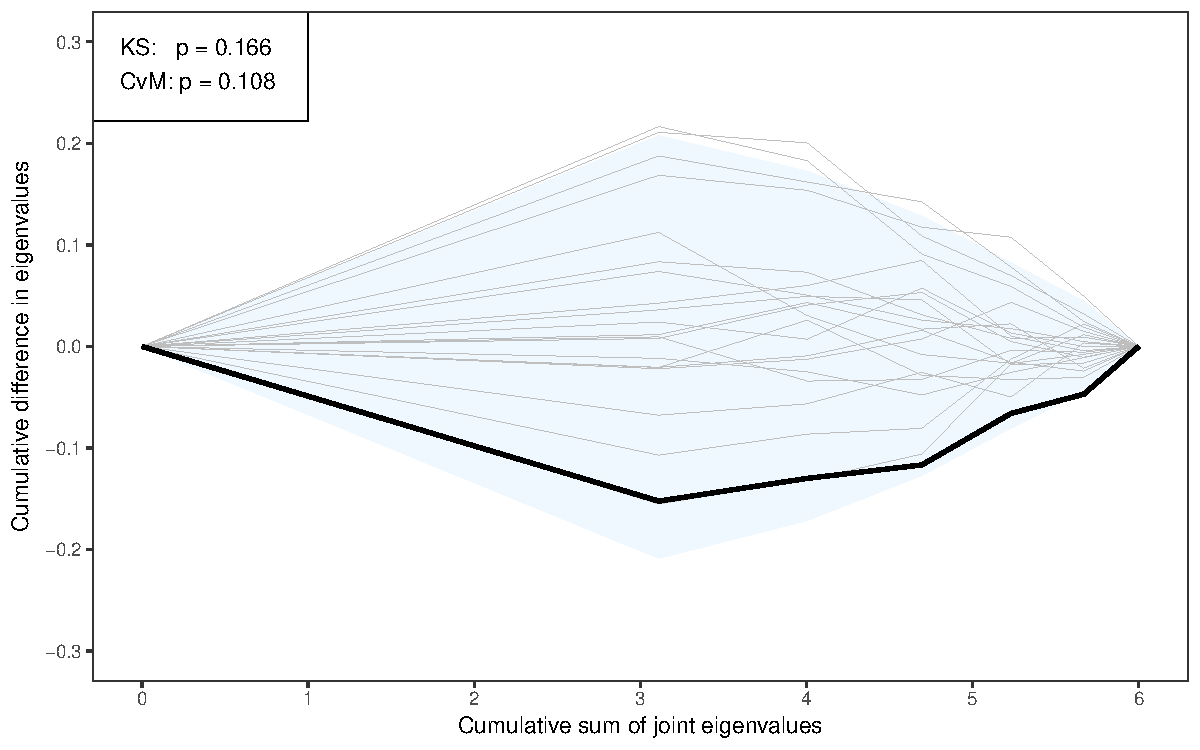
\includegraphics[scale = 0.3]{essDKSEce.pdf}
\end{figure}
\small
Annotations: $p$-values from two test statistics:
\begin{itemize}
\item Kolmogorov-Smirnov: $\max_{k=1,\dotsc,d} \bigg\lvert \sum_{j=1}^k \lambda^1_j -  \lambda^2_j \bigg\rvert$
\item Cramér-von Mises: $\sum_{k=1}^{d-1} \frac{\lambda_k + \lambda_{k+1}}{2} \bigg( \sum_{j=1}^k \lambda^1_j - \lambda^2_j  \bigg)^2$
\end{itemize}
\end{frame}

\subsection{The hair plot}
\begin{frame}
\frametitle{The hair plot}
   \begin{itemize}
   \item Let $\lambda_\text{max} = \max\{\lambda^1_1, \lambda^2_1\}$. 
   \item Define $\mu_{jk} = \sqrt{\frac{\lambda^1_k}{\lambda_\text{max}}} \left|(\eta^1_k)^\top \eta^2_j \right|$, $\nu_{jk} = \sqrt{\frac{\lambda^2_j}{\lambda_\text{max}}} \left|(\eta^2_j)^\top \eta^1_k \right|$,
   $\theta_{jk} = \arccos \left( \left|(\eta^1_k)^\top \eta^2_j \right| \right)$
   \item In the $jk$th position in a $d \times d$ grid, draw two arrows (hairs): 
   \begin{itemize}
   	\item A blue arrow with length $\mu_{jk}$ drawn at an angle of $\theta_{jk}$ counter-clockwise from the diagonal
   	\item A red arrow with length $\mu_{jk}$ drawn at an angle of $\theta_{jk}$ clockwise from the diagonal
   \end{itemize} 
  \item Note: If $\eta^1_k \perp \eta^2_j$, then $\mu_{jk} = \nu_{jk} =  0$. If $\eta^1_k = \eta^2_j$, then $\theta_{jk} = \arccos(1) = 0$ (due to unit length). 
  \item Thus: Identical structures imply zero-length arrows for $j \neq k$ and identical red and blue arrows at the diagonal for $j = k$.  
   \end{itemize}
\end{frame}

\begin{frame}
\frametitle{The hair plot}
\begin{figure}
\centering
    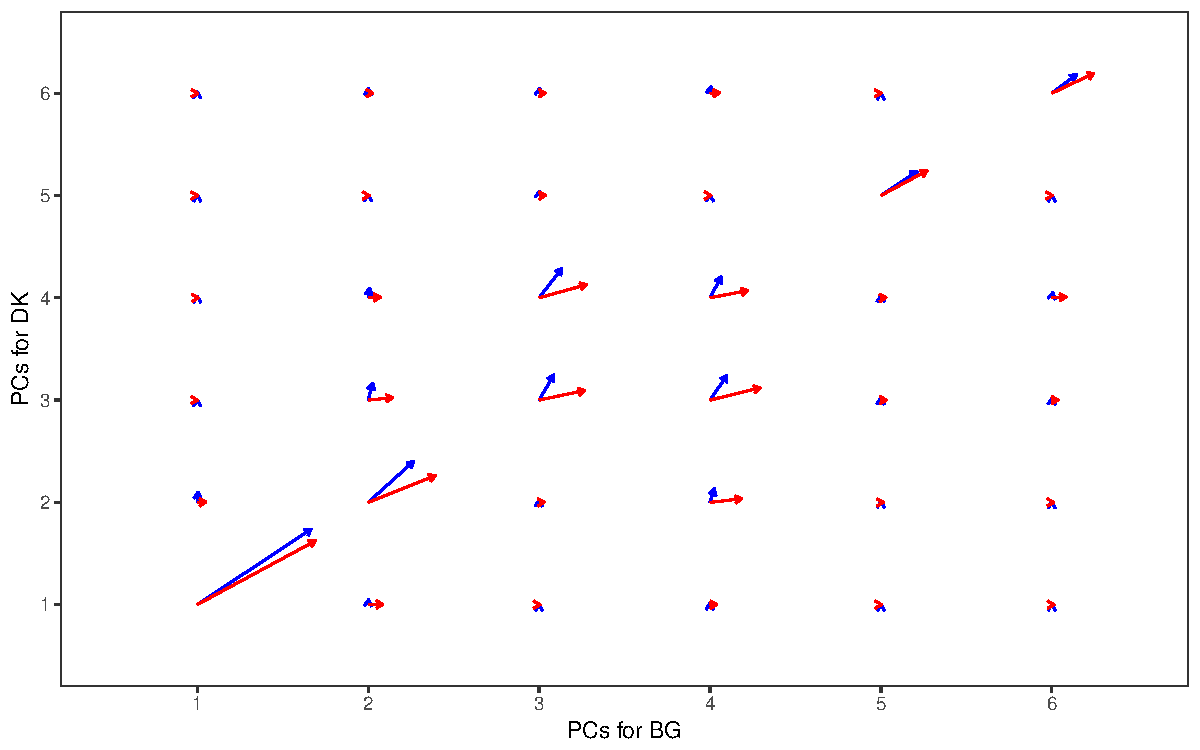
\includegraphics[scale = 0.4]{essDKBGhair.pdf}
\end{figure}
\end{frame}

\subsection{The pancake plot}
\begin{frame}
\frametitle{The pancake plot}
For $k \in \{1, 2\}$, do:
   \begin{itemize}
   \item[2.] For $i \in 1, ..., d$, normalize $\eta^k_i$ and add a bar to the plot consisting of differently colored "pancakes" whose widths correspond to their standardized loading weights. 
   \item[3.] Annotate each bar with the amount of (cumulated) explained variance when using the information from this and the previous components, i.e. 
   $$\frac{\sum_{j = 1}^i \eta^k_j}{\sum_{j=1}^d \eta^k_j}$$
   % \grey{\quad \left(\text{or } \frac{ \eta^k_j}{\sum_{j=1}^d \eta^k_j} \right) } 
   \end{itemize}   
\end{frame}

\begin{frame}
\frametitle{The pancake plot}
    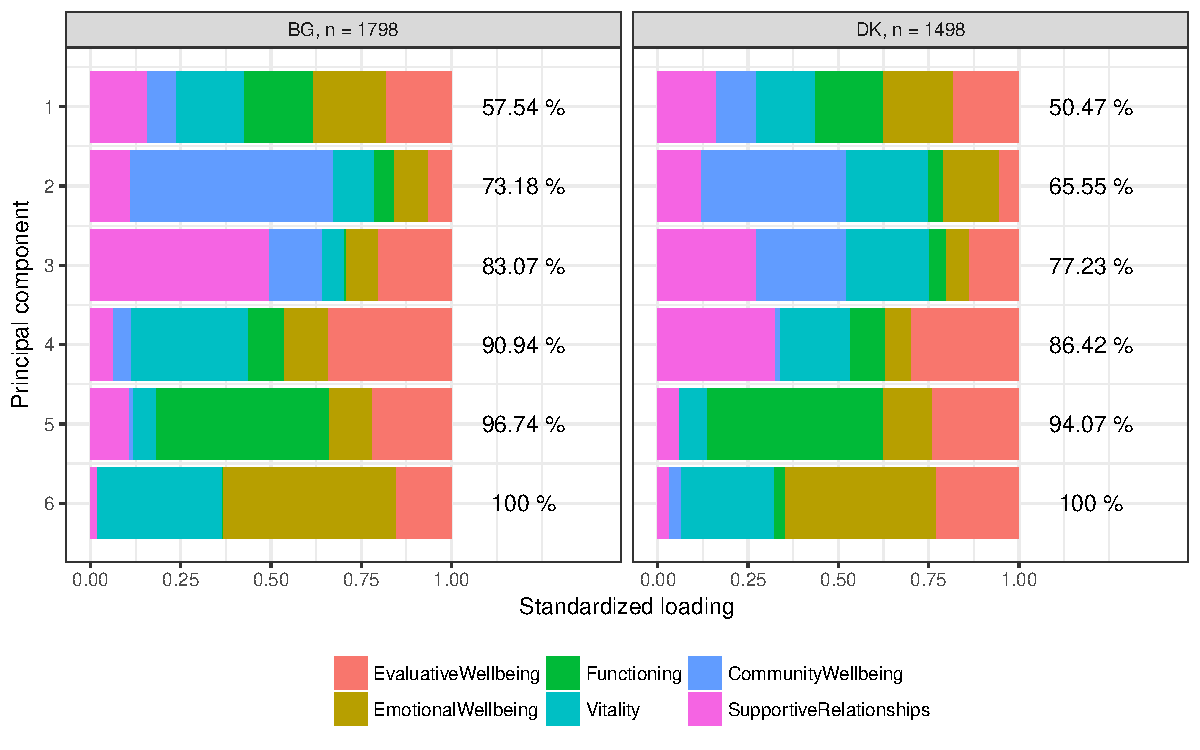
\includegraphics[scale = 0.5]{essDKBGpancake.pdf}
\end{frame}

\section{Data example}
\subsection{setup}
\begin{frame}
\frametitle{Data example - set-up}
\begin{itemize}
\item Data on psychological well-being from the 2012 version of the European Social Survey (ESS)
\item We use 35 items for producing 6 distinct psychological well-being scales
\item ESS report: Bulgaria (BG) and Denmark (DK) are particularly different in the interplay between different aspects of psychological well-being (evaluated at aggregated country-level)
\item Postulate: Denmark and Sweden (SE) are quite similar in what defines personal happiness and psychological well-being
\item Strategy: Run all three methods on the DK vs. BG and DK vs. SE comparisons and expect to find \textit{different} data structures for DK vs. BG and \textit{similar} structures for DK vs. SE
\item Only use complete cases. This results in $n_\text{DK} = 1498$, $n_\text{BG} = 1798$ and $n_\text{SE} = 1736$ observations, respectively. 
\end{itemize}
\end{frame}

\subsection{DK vs. BG}
\begin{frame}
\frametitle{DK vs. BG: CE plot}
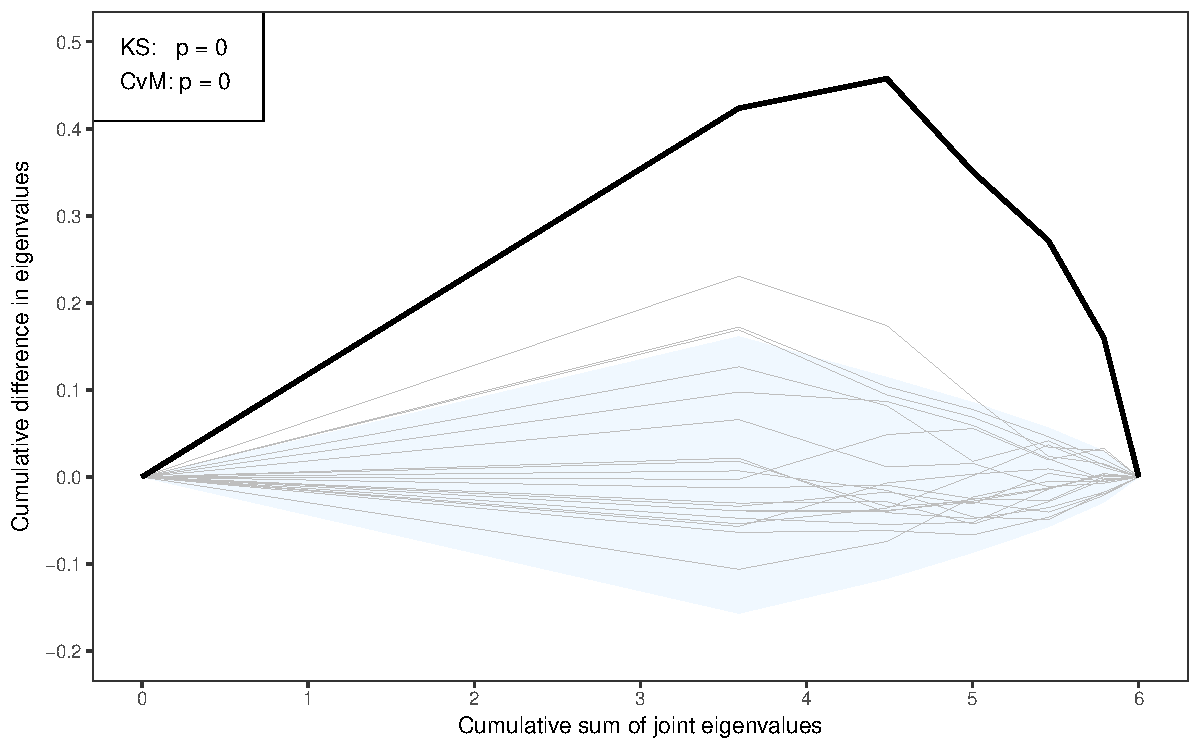
\includegraphics[scale = 0.5]{essDKBGce.pdf}
\end{frame}

\begin{frame}
\frametitle{DK vs. BG: hair plot}
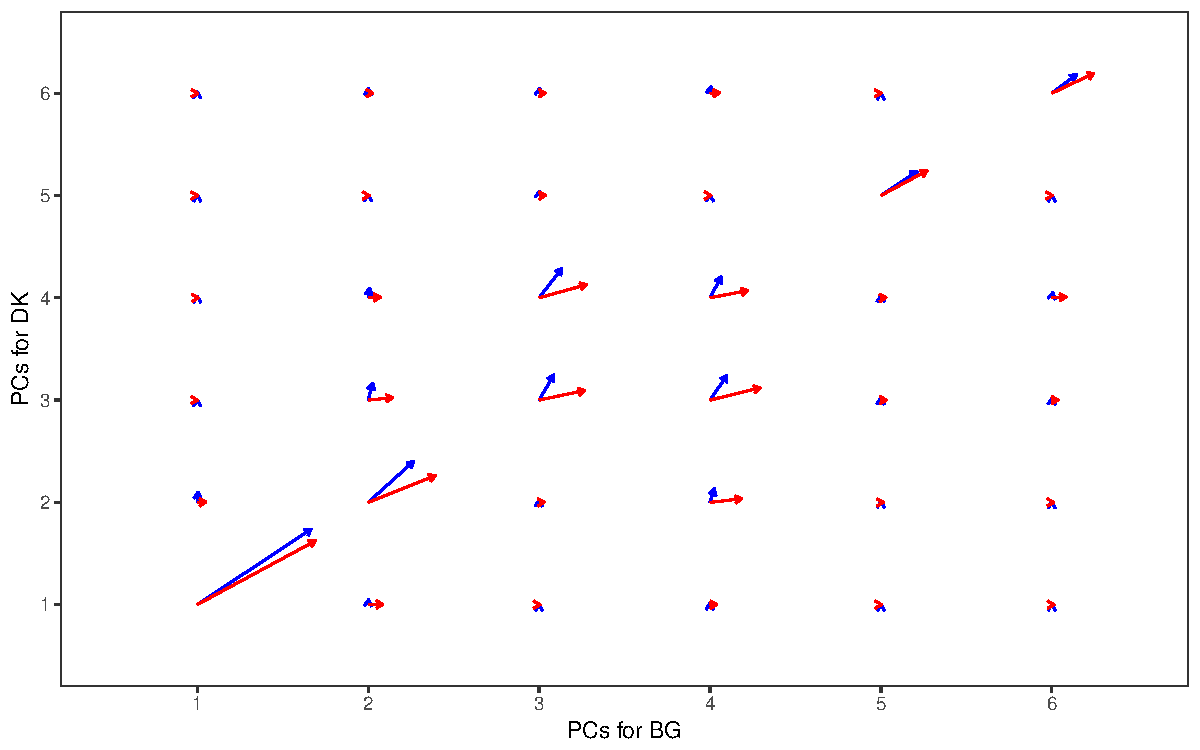
\includegraphics[scale = 0.5]{essDKBGhair.pdf}
\end{frame}

\begin{frame}
\frametitle{DK vs. BG: Pancake plot}
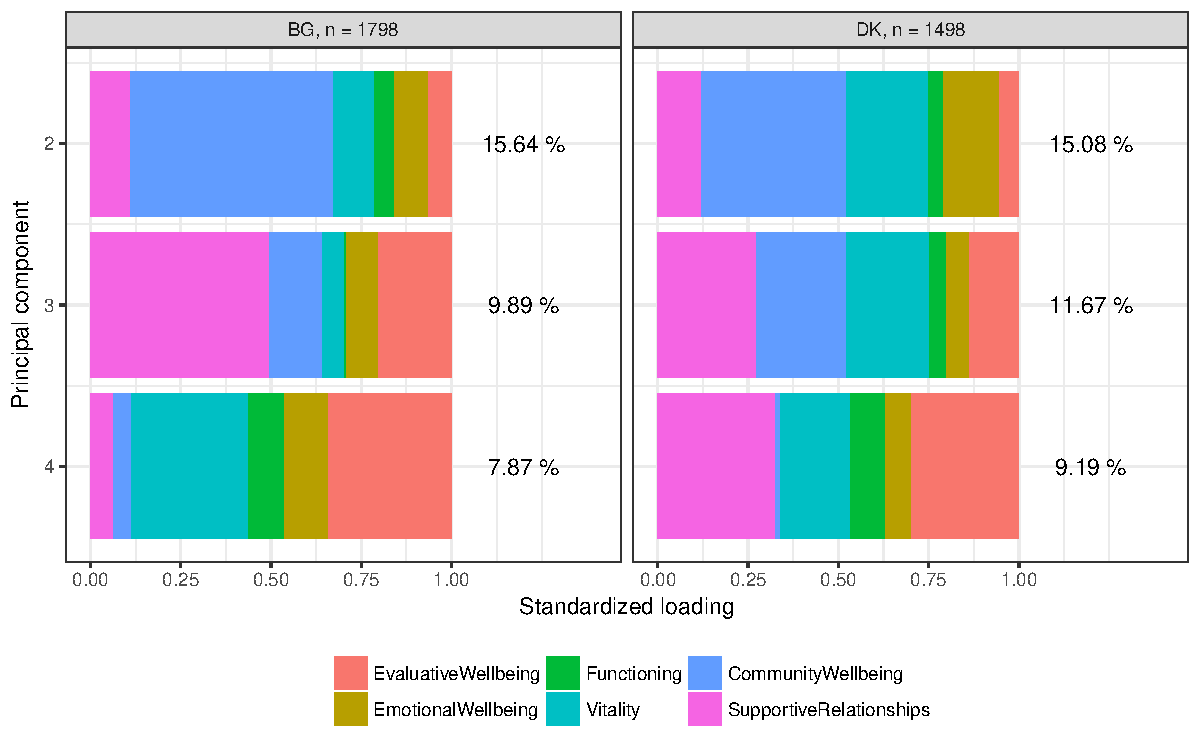
\includegraphics[scale = 0.5]{essDKBGpancake234.pdf}
\end{frame}

\begin{frame}
\frametitle{DK vs. BG: Pancake Wally plot}
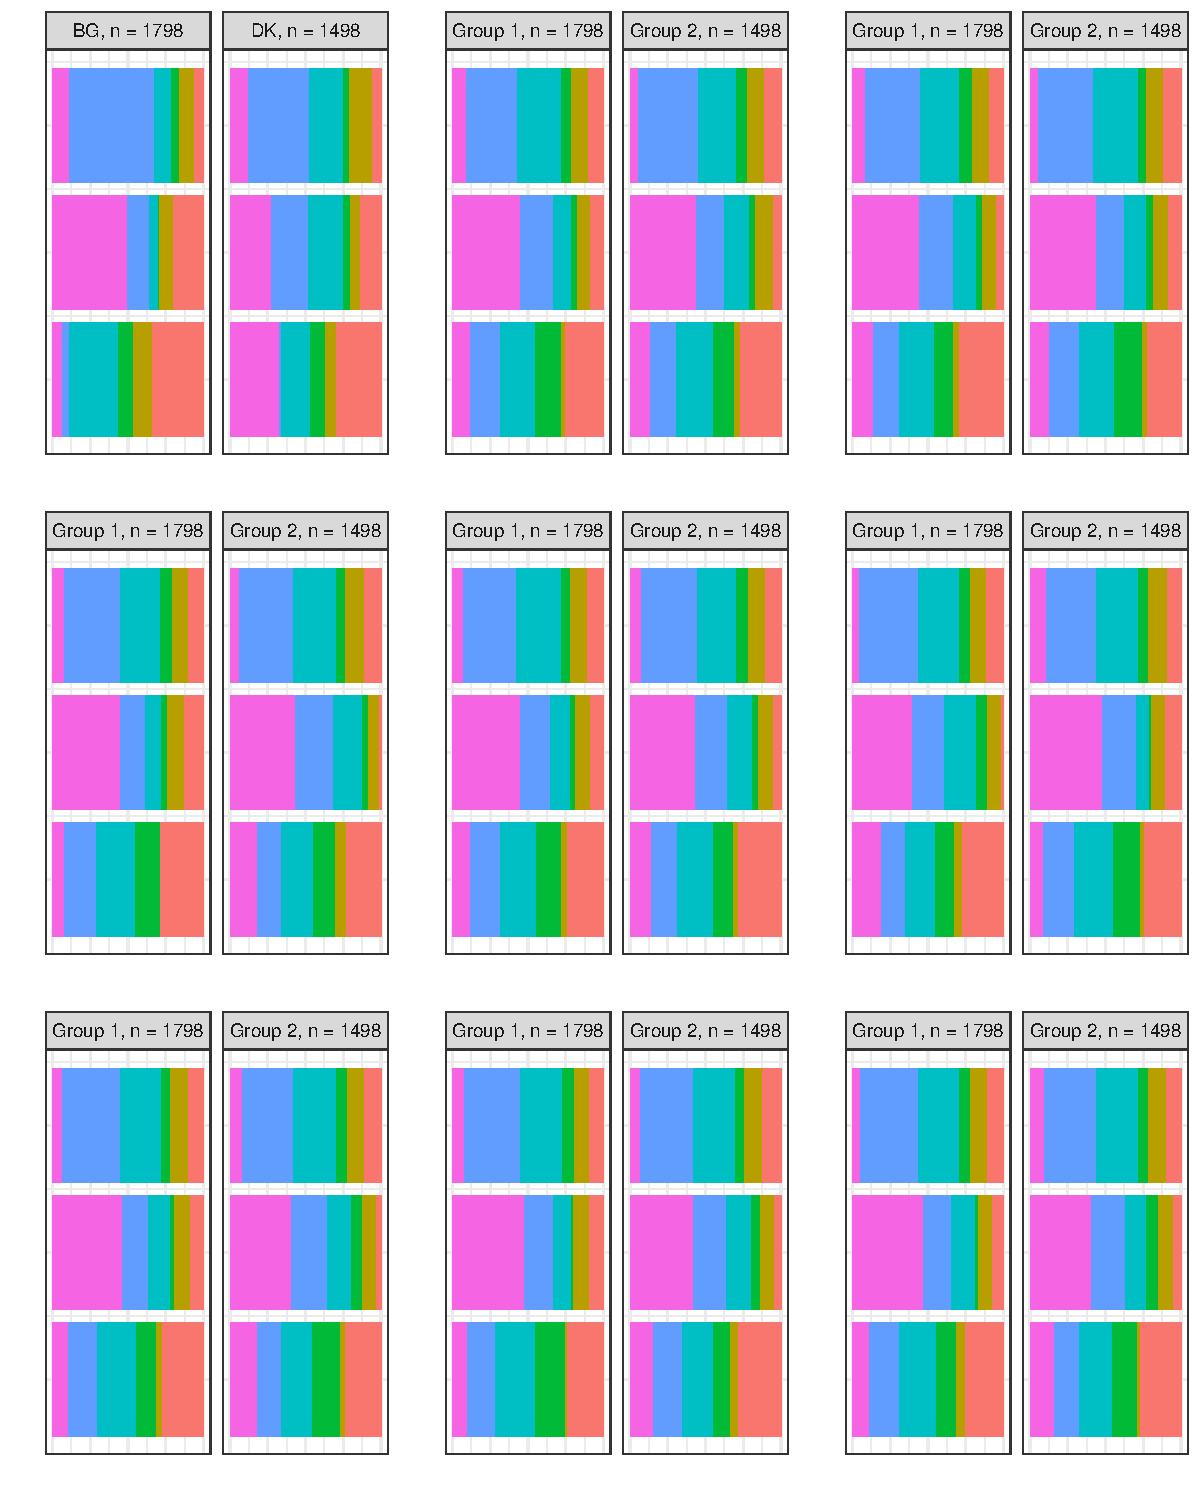
\includegraphics[scale = 0.4]{essDKBGWallyPCADSC234.pdf}
\end{frame}

\subsection{DK vs. SE}
\begin{frame}
\frametitle{DK vs. SE: CE plot}
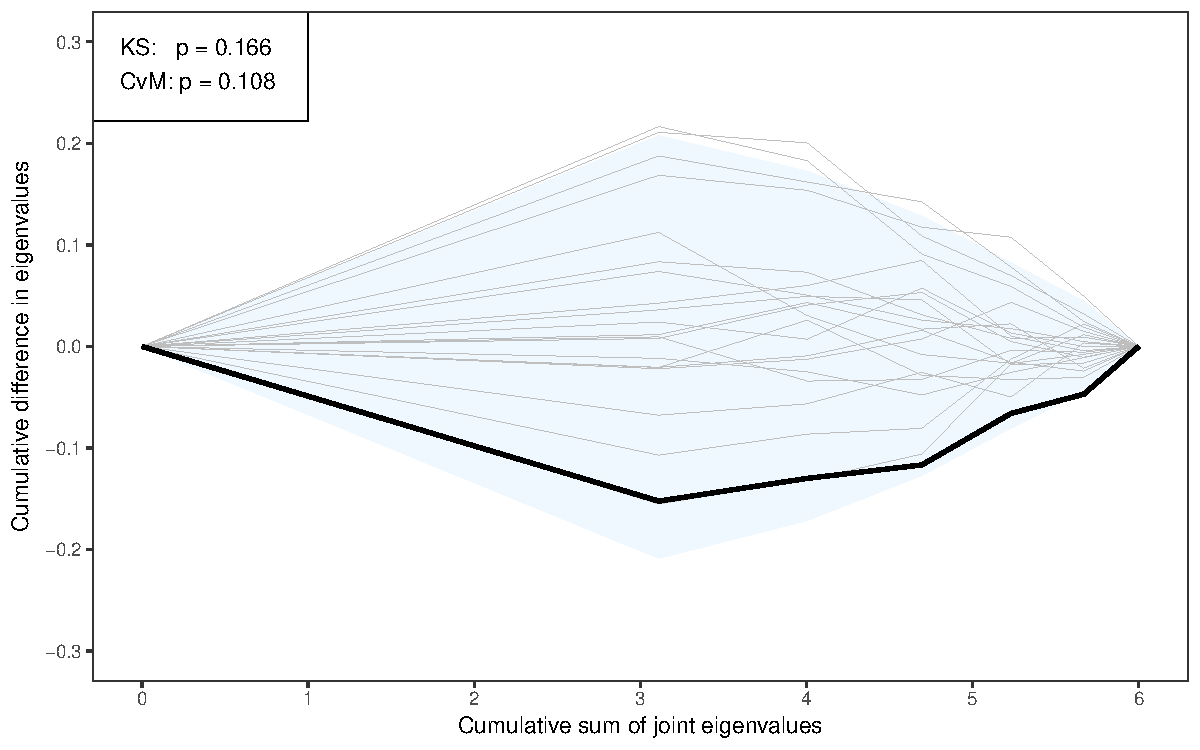
\includegraphics[scale = 0.5]{essDKSEce.pdf}
\end{frame}

\begin{frame}
\frametitle{DK vs. SE: hair plot}
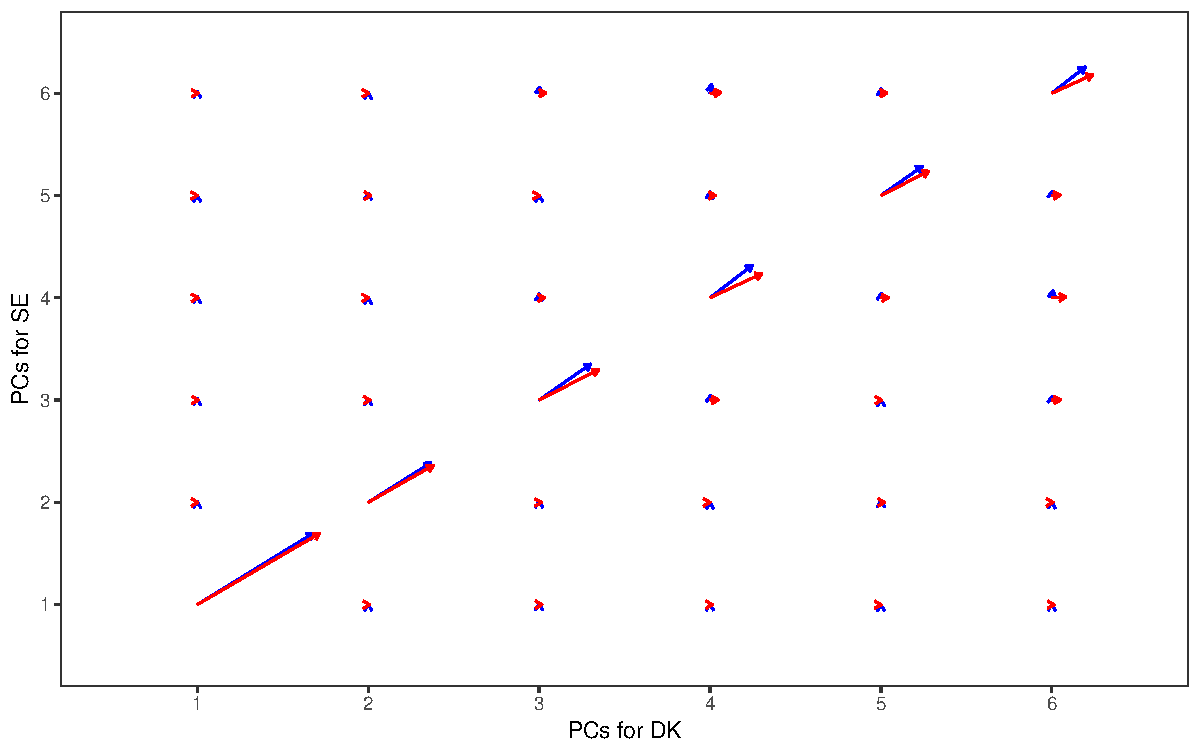
\includegraphics[scale = 0.5]{essDKSEhair.pdf}
\end{frame}

\begin{frame}
\frametitle{DK vs. SE: Pancake plot}
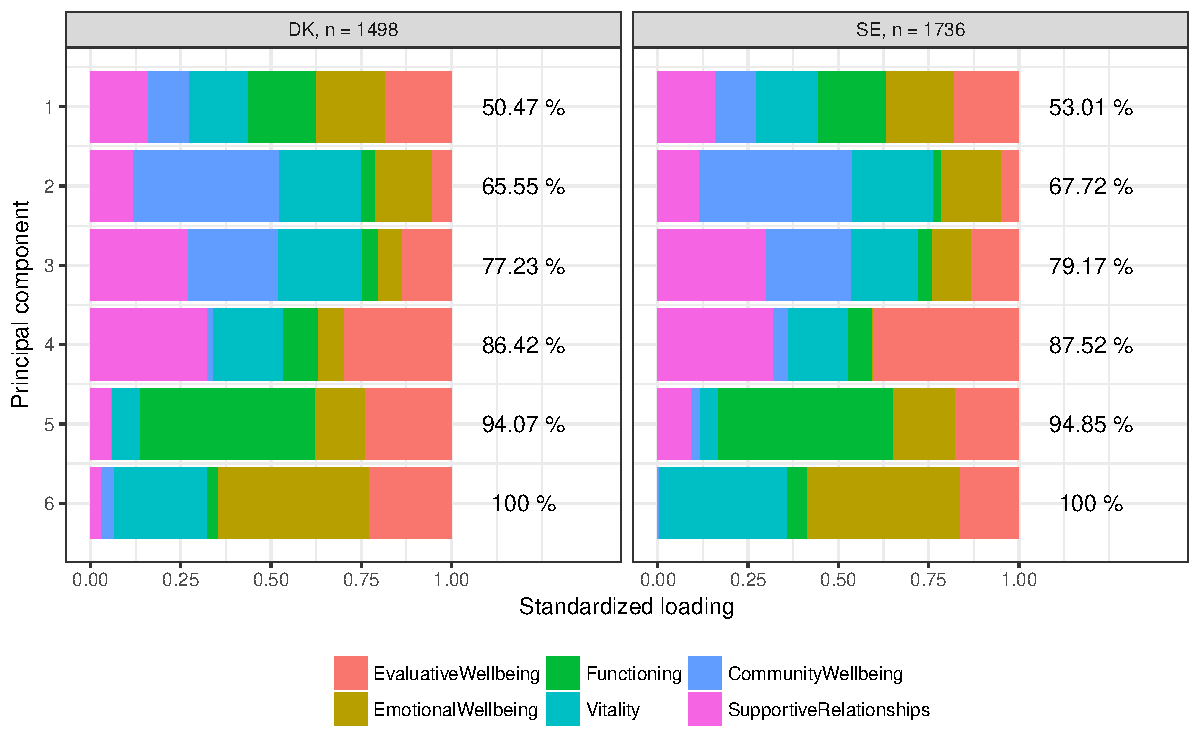
\includegraphics[scale = 0.5]{essDKSEpancake.pdf}
\end{frame}

\begin{frame}
\frametitle{DK vs. SE: Pancake Wally plot}
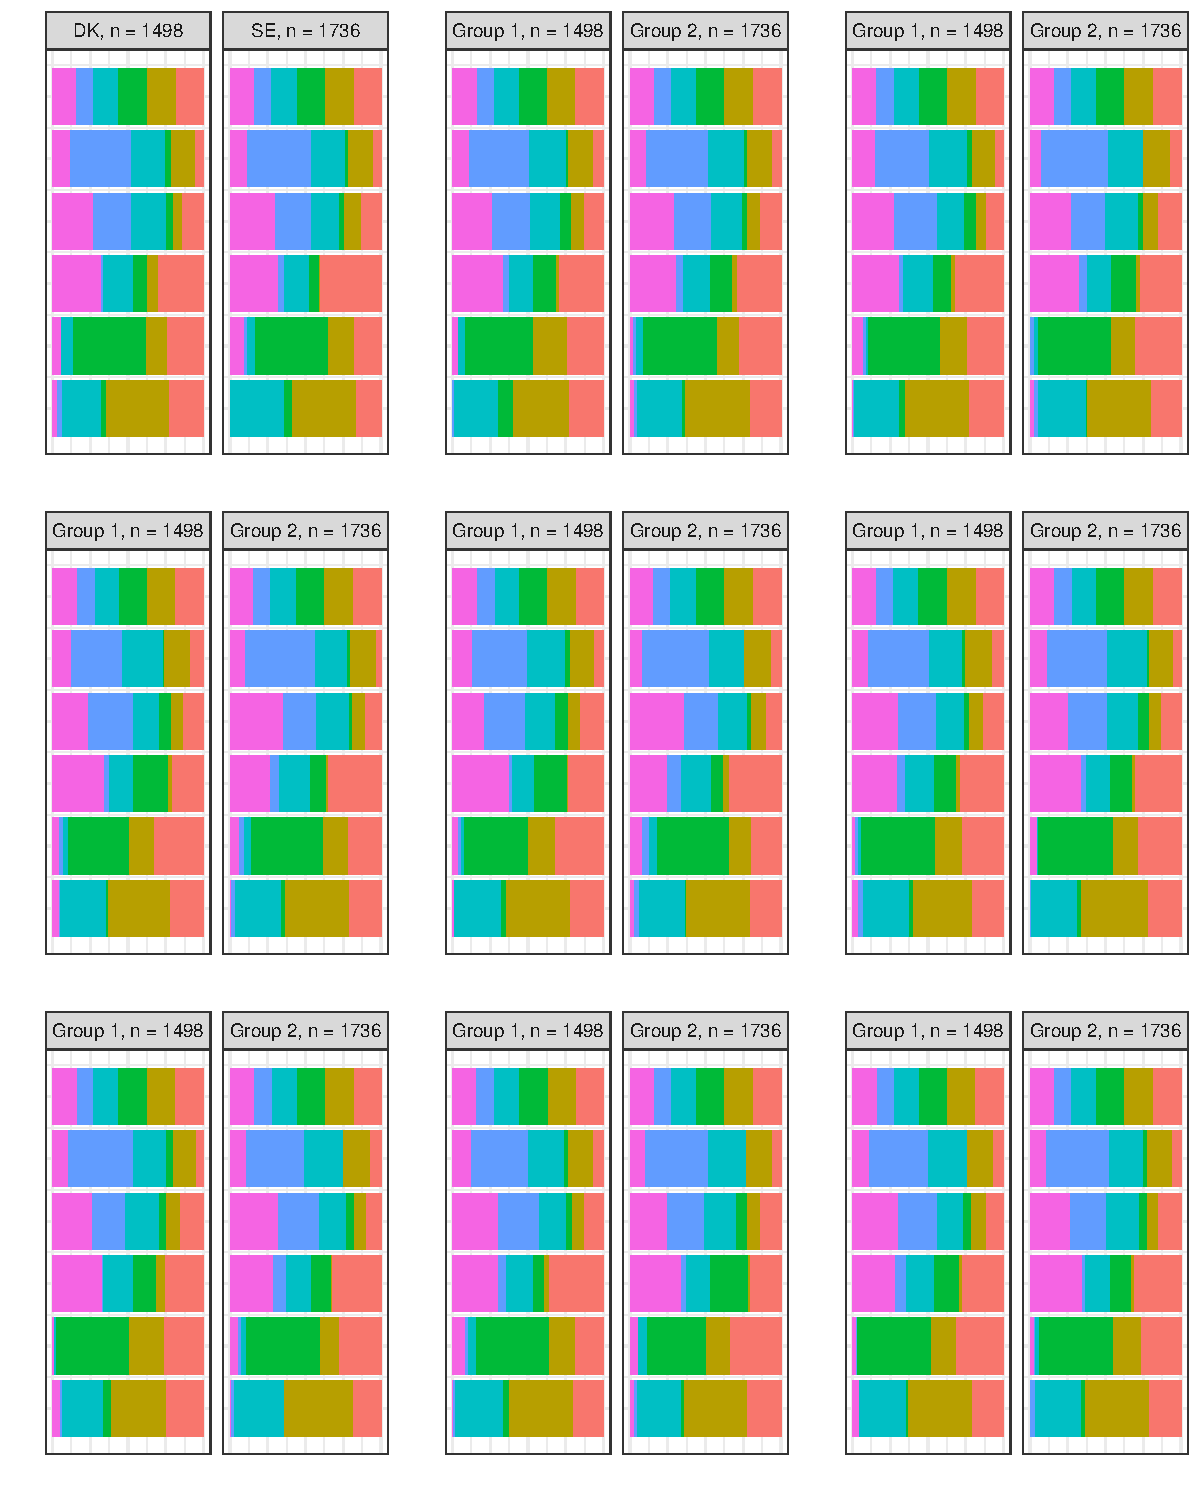
\includegraphics[scale = 0.4]{essDKSEWallyPCADSC.pdf}
\end{frame}

\section{Next steps}
\begin{frame}
\frametitle{Ideas for next steps}
\begin{itemize}
\item Investigate sensitivity towards the sample sizes $n_1$ and $n_2$
\item Limitations: What sorts of problems can never be found using PCADSC? 
\begin{itemize}
\item Differences in scaling, as we standardize all variables
\item More?
\end{itemize}
\item Interpretation for binary variables?
\item Any meaningful way to allow for nominal, categorical variables?
\item ... ?
\end{itemize}

\end{frame}

\end{document} 